\documentclass[dvipdfmx]{beamer}
\usepackage{tutorial}

\title{計算機実験(L7) --- 最適化問題・スーパーコンピューターと計算物理}
\date{2016/06/29}

\begin{document}

\begin{frame}
  \titlepage
  \tableofcontents
\end{frame}

\section{最適化問題}

\begin{frame}[t,fragile]{最適化問題}
  \begin{itemize}
    %\setlength{\itemsep}{1em}
  \item 目的関数$f(x)$の最小値(あるいは最大値)とその場所を求めたい
    \begin{itemize}
    \item 連続最適化問題
    \item 離散最適化(組み合わせ最適化)問題 $\Leftarrow$ 難しい
    \end{itemize}
  \item 真の(大局的な)最小値(最大値)を求めるのは難しい
  \item 一般的には極値を求めることしかできない
  \item 多次元では極小を囲い込むことができない
  \item 導関数を使う方法: ニュートン法、最急降下法、共役勾配法、準ニュートン法
  \item 使わない方法: 囲い込み法、Nelder-Meadの滑降シンプレックス法、シミュレーテッド・アニーリング
  \end{itemize}
\end{frame}

\section{ニュートン法}

\begin{frame}[t,fragile]{ニュートン法}
  \begin{itemize}
    \setlength{\itemsep}{1em}
  \item 反復法により方程式$f(x)=0$の解を求める
  \item 真の解を$x_0$、現在の解の候補を$x_n=x_0+\epsilon$とすると
    \[
    0 = f(x_0) = f(x_0+\epsilon-\epsilon) = f(x_n) - f'(x_n) \epsilon + O(\epsilon^2)
    \]
  \item 次の解の候補 (反復法、逐次近似法)
    \[
    \epsilon \approx \frac{f(x_n)}{f'(x_n)} \quad\quad x_{n+1} = x_n - \frac{f(x_n)}{f'(x_n)}
    \]
  \item 複素変数の複素関数や多変数の場合にも自然に拡張可
  \end{itemize}
\end{frame}

\begin{frame}[t,fragile]{ニュートン法の収束}
  \begin{itemize}
    \setlength{\itemsep}{1em}
  \item $x_n$が$x_0$に十分近い時
    \begin{align*}
      f(x_n) &\approx f'(x_0) (x_n-x_0) + f''(x_0) \frac{(x_n - x_0)^2}{2} \\
      f'(x_n) &\approx f'(x_0) + f''(x_0) (x_n - x_0)
    \end{align*}
  \item ニュートン法で一回反復すると
    \begin{align*}
      x_{n+1} =  x_n - \frac{f(x_n)}{f'(x_n)} &\approx x_n - (1-\frac{f''(x_0)}{f'(x_0)}\frac{(x_n-x_0)}{2})(x_n-x_0) \\
      (x_{n+1}-x_0) &\approx \frac{f''(x_0)}{2f'(x_0)} (x_n - x_0)^2
    \end{align*}
    \item 一回の反復で誤差が2乗で減る(正しい桁数が倍に増える) ⇒ 二次収束
  \end{itemize}
\end{frame}

\begin{frame}[t,fragile]{多次元の場合}
  \begin{itemize}
    \setlength{\itemsep}{1em}
  \item $f(x)=0$: $d$次元(非線形)連立方程式
  \item $x$は$d$次元のベクトル: $x = (x_1,x_2,\cdots,x_d)$
  \item $f(x)$も$d$次元のベクトル: $f(x) = (f_1(x), f_2(x),\cdots,f_d(x))$
  \item 真の解のまわりでの展開 ($x_n = x_0 + \epsilon$)
    \[
    0 = f(x_0) = f(x_0+\epsilon-\epsilon) = f(x_n) - \frac{\partial f(x_n)}{\partial x} \cdot \epsilon + O(|\epsilon|^2)
    \]
  \item ヤコビ行列($d\times d$): $\displaystyle \Big(\frac{\partial f(x_n)}{\partial x}\Big)_{ij} = \frac{\partial f_i(x_n)}{\partial x_j}$
  \item 次の解の候補: $\displaystyle x_{n+1} = x_n - \Big(\frac{\partial f(x_n)}{\partial x}\Big)^{-1} f(x_n)$
  \end{itemize}
\end{frame}

\begin{frame}[t,fragile]{ニュートン法による最適化}
  \begin{itemize}
    \setlength{\itemsep}{1em}
  \item $x$は$d$次元のベクトル: $x = (x_1,x_2,\cdots,x_d)$, $g(x)$はスカラー
  \item 勾配ベクトル: $\displaystyle (\nabla g(x))_i = \frac{\partial g(x)}{\partial x_i}$
  \item 極小値(最小値)となる条件: $\nabla g(x)=0$
  \item ニュートン法で$f(x)$を$\nabla g(x)$で置き換えればよい
  \item 次の解の候補: $\displaystyle x_{n+1} = x_n - H^{-1}(x_n) \nabla g(x_n)$
  \item ヘッセ行列(Hessian): $\displaystyle H_{ij}(x_n) = \frac{\partial^2 g}{\partial x_i \partial x_j}(x_n)$
  \end{itemize}
\end{frame}

\begin{frame}[t,fragile]{準ニュートン法}
  \begin{itemize}
    %\setlength{\itemsep}{1em}
  \item ニュートン法では、ヘッセ行列の計算・保存が必要
  \item 準ニュートン法: それまでの反復で計算した勾配ベクトルから、ヘッセ行列を近似($B_n$)
  \item BFGS法(Broyden-Fletcher-Goldfarb-Shanno)
    \[
    B_{n+1} = B_{n} + \frac{y_n y_n^T}{y_n^T s_n} - \frac{B_{n} s_n (B_{n} s_n)^T}{s_n^T B_n s_n}
    \]
  \item $s_n = x_{n+1} - x_n$、$y_n = \nabla g(x_{n+1}) - \nabla g(x_n)$
  \item 直接$B_{n}$の逆行列$C_{n}$を更新することも可能
    \[
    C_{n+1} = B_{n+1}^{-1} = C_n + \Big( 1 + \frac{y_n^T C_n y_n}{y_n^T s_n} \Big)
    \frac{s_n s_n^T}{y_n^T s_n} - \frac{C_n y_n s_n^T + s_n y_n^T C_n^T}{y_n^T s_n} \]
  \item 他にも、SR1法、BHHH法、記憶制限BFGS法
  \end{itemize}
\end{frame}

\section{囲い込み法}

\begin{frame}[t,fragile]{囲い込み法(一次元の最適化)}
  \begin{itemize}
    \setlength{\itemsep}{1em}
  \item $f(a) > f(b) < f(c)$を満たす3点の組$a < b < c$の領域を狭めていく
  \item $[a,b]$、$[b,c]$の広い方(例えば後者)を$b$から見て
    $0.382:0.618$ (黄金比)に内分する点を$x$とする
    \begin{itemize}
    \item $f(b) > f(x)$の場合: $[b,c]$を新しい領域にとる
    \item $f(b) < f(x)$の場合: $[a,x]$を新しい領域にとる
    \end{itemize}
  \item もともとの$b$が$[a,c]$を$0.382:0.618$に内分する点だった場合、
    新しい領域の幅は、どちらの場合も0.618
  \item 最初の比率が黄金比からずれていたとしても、黄金比に収束
  \end{itemize}
\end{frame}

\begin{frame}[t,fragile]{最初の囲い込み}
  \begin{itemize}
    \setlength{\itemsep}{1em}
  \item 1点を選び、適当な$\Delta x$を取る
  \item 左右に$\Delta x$動かしてみて、関数値が小さくなる方へ動く
  \item どちらに進んでも関数値が大きくなる場合には、囲い込み完了
  \item 小さくなった場合、その方向へ再び増えるまで$\Delta x$を倍々に増やしながら進む
  \item 最後の3点で極小値を囲い込むことができる
  \end{itemize}
\end{frame}

\begin{frame}[t,fragile]{極小値をとる$x$の精度}
  \begin{itemize}
    \setlength{\itemsep}{1em}
  \item 実数の有効桁数を16桁($\epsilon \approx 10^{-16}$)とする(倍精度)
  \item 真の極小($x_0$)のまわりでテイラー展開
    \[
    f(x) \approx f(x_0) + \frac{1}{2} f''(x_0) (x-x_0)^2
    \]
  \item $f''(x_0) / f(x_0)$が$O(1)$だとすると
    \[
    |x-x_0| \sim \sqrt{\epsilon} \sim 10^{-8}
    \]
    以下になると、第二項の第一項に対する比が$\epsilon$よりも小さくなる
  \item それ以上領域を狭めても、関数値は変化しない
  \end{itemize}
\end{frame}

\section{最急降下法と勾配降下法}

\begin{frame}[t,fragile]{最急降下法(steepest descent)}
  \begin{itemize}
    \setlength{\itemsep}{1em}
  \item 関数の微分の情報を使う
  \item 現在の点$\bf x$における勾配を計算
    \[
    -\nabla f|_i = -\frac{\partial f}{\partial x_i}
    \]
  \item 坂を下る方向にそって、一次元最適化
  \item 動いた先の勾配の方向でさらに最適化を繰り返す
  \item 関数値は単調減少 $\Rightarrow$ 極小値に収束
  \end{itemize}
\end{frame}

\begin{frame}[t,fragile]{勾配降下法(gradient descent)}
  \begin{itemize}
    \setlength{\itemsep}{1em}
  \item 勾配方向に一次元最適化を行うかわりに、あらかじめ決めた一定量($\epsilon$)だけ坂を下る
    \[
    x_{n+1} = x_n - \epsilon \, \nabla f
    \]
  \item あらかじめ最適な$\epsilon$を知るのは困難
  \item 機械学習の分野では、(なぜか) $\epsilon=0.1$が良いとされている
  \item この方法を「最急降下法」、一次元最適化を行う勾配法を「最適降下法(optimum descent)」と呼ぶ場合も
  \item c.f.) 確率的勾配降下法(stochastic gradient descent)
  \end{itemize}
\end{frame}

\begin{frame}[t,fragile]{制約条件付きの場合}
  \begin{itemize}
    % \setlength{\itemsep}{1em}
  \item 目的関数: $f(x)$
  \item 制約条件:
    \begin{itemize}
    \item $g_i(x) = 0$ \ ($i=1,\cdots,m$) \ (等式制約条件)
    \item $h_j(x) \ge 0$ \ ($j=1,\cdots,n$) \ (不等式制約条件)
    \end{itemize}
  \item 等式制約条件の付いている場合: Lagrangeの未定乗数法
    \[
    L(x,\lambda_1,\cdots,\lambda_m)=f(x)+\sum_i \lambda_i g_i(x)
    \]
    を考え、$x,\lambda_1,\cdots,\lambda_m$の微分が零となる点を探す
  \item 不等式制約条件の付いている場合: c.f. 線形計画法, ペナルティ関数法
  \end{itemize}
\end{frame}

\begin{frame}[t,fragile]{細長い谷の場合}
  \vspace*{1em}
  \hspace*{1em}\resizebox{1\textwidth}{!}{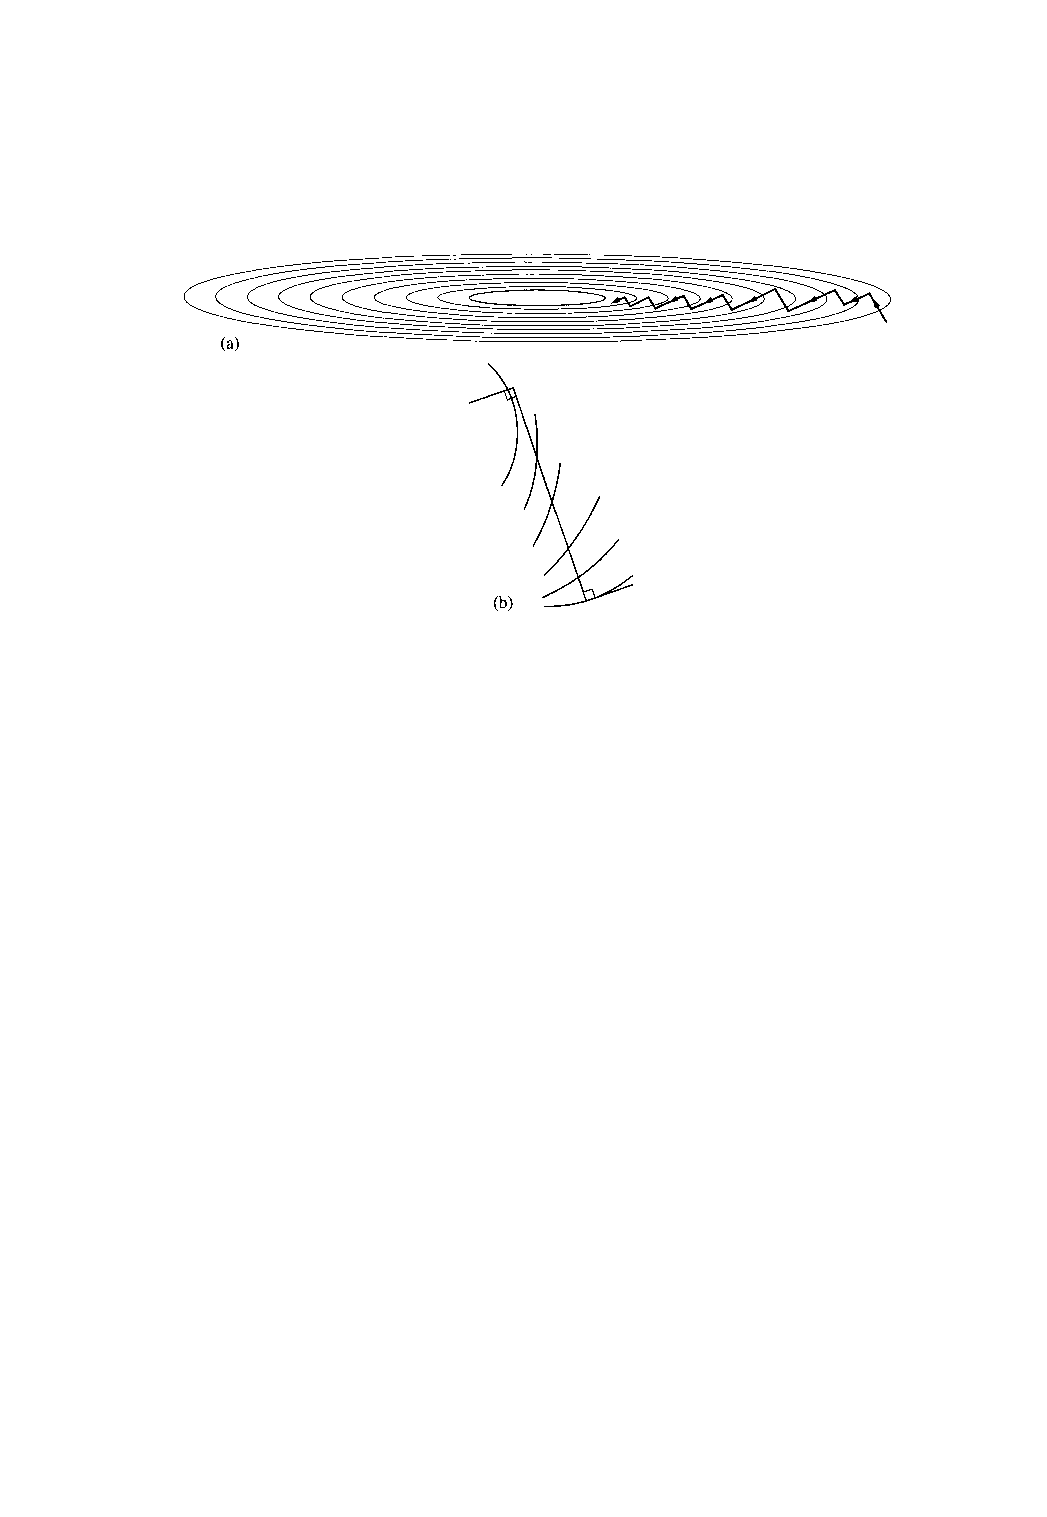
\includegraphics{image/steepest-descent.pdf}}

  \vspace*{-2em}
  \hspace*{20em}{\footnotesize(Press et al 1988)}
\end{frame}

\section{Nelder-Meadの滑降シンプレックス法}

\begin{frame}[t,fragile]{Nelder-Meadの滑降シンプレックス法}
  \begin{itemize}
    \setlength{\itemsep}{1em}
  \item 関数値のみ。導関数の情報を必要としない
  \item プログラミングが簡単
  \item 収束は遅いが、安定に極小値が求まる
  \item $N+1$個の頂点からなる$N$次元の単体(シンプレックス)を変形しながら、極小値を探す
    \begin{itemize}
    \item 2次元: 三角形
    \item 3次元: 四面体
    \end{itemize}
  \item 別名「アメーバ法」
  \end{itemize}
\end{frame}

\begin{frame}[t,fragile]{Nelder-Meadの滑降シンプレックス法}
  \begin{itemize}
    \setlength{\itemsep}{1em}
  \item $N+1$個の点$x_0,x_1,\cdots,x_N$は$f(x_0) \le f(x_1) \le \cdots \le f(x_N)$と並べられているとする
  \item 最大値を取る点$x_N$を除く$N$点の重心を$x_g$とする
  \item Nelder-Mead法では以下のステップを繰り返す
    \begin{itemize}
      \item $x_N$の$x_g$に関する対称な点と$x_N$の関数値を比較し、小さい方に移動(反射)
      \item $x_0$の関数値よりも小さくなるようであればさらに先に進む(拡大)
      \item $x_N$の関数値が$x_{N-1}$のものよりもまだ大きい場合には$x_N$を$x_g$に近づける(縮小)
      \item それでも$x_N$の関数値が小さくならない場合、$x_0$以外の点を$x_0$に一様に近づける(収縮)
    \end{itemize}
  \end{itemize}
\end{frame}

\begin{frame}[t,fragile]{Nelder-Meadの滑降シンプレックス法}
  \vspace*{-2em}
  \hspace*{1em}\resizebox{!}{1.0\textheight}{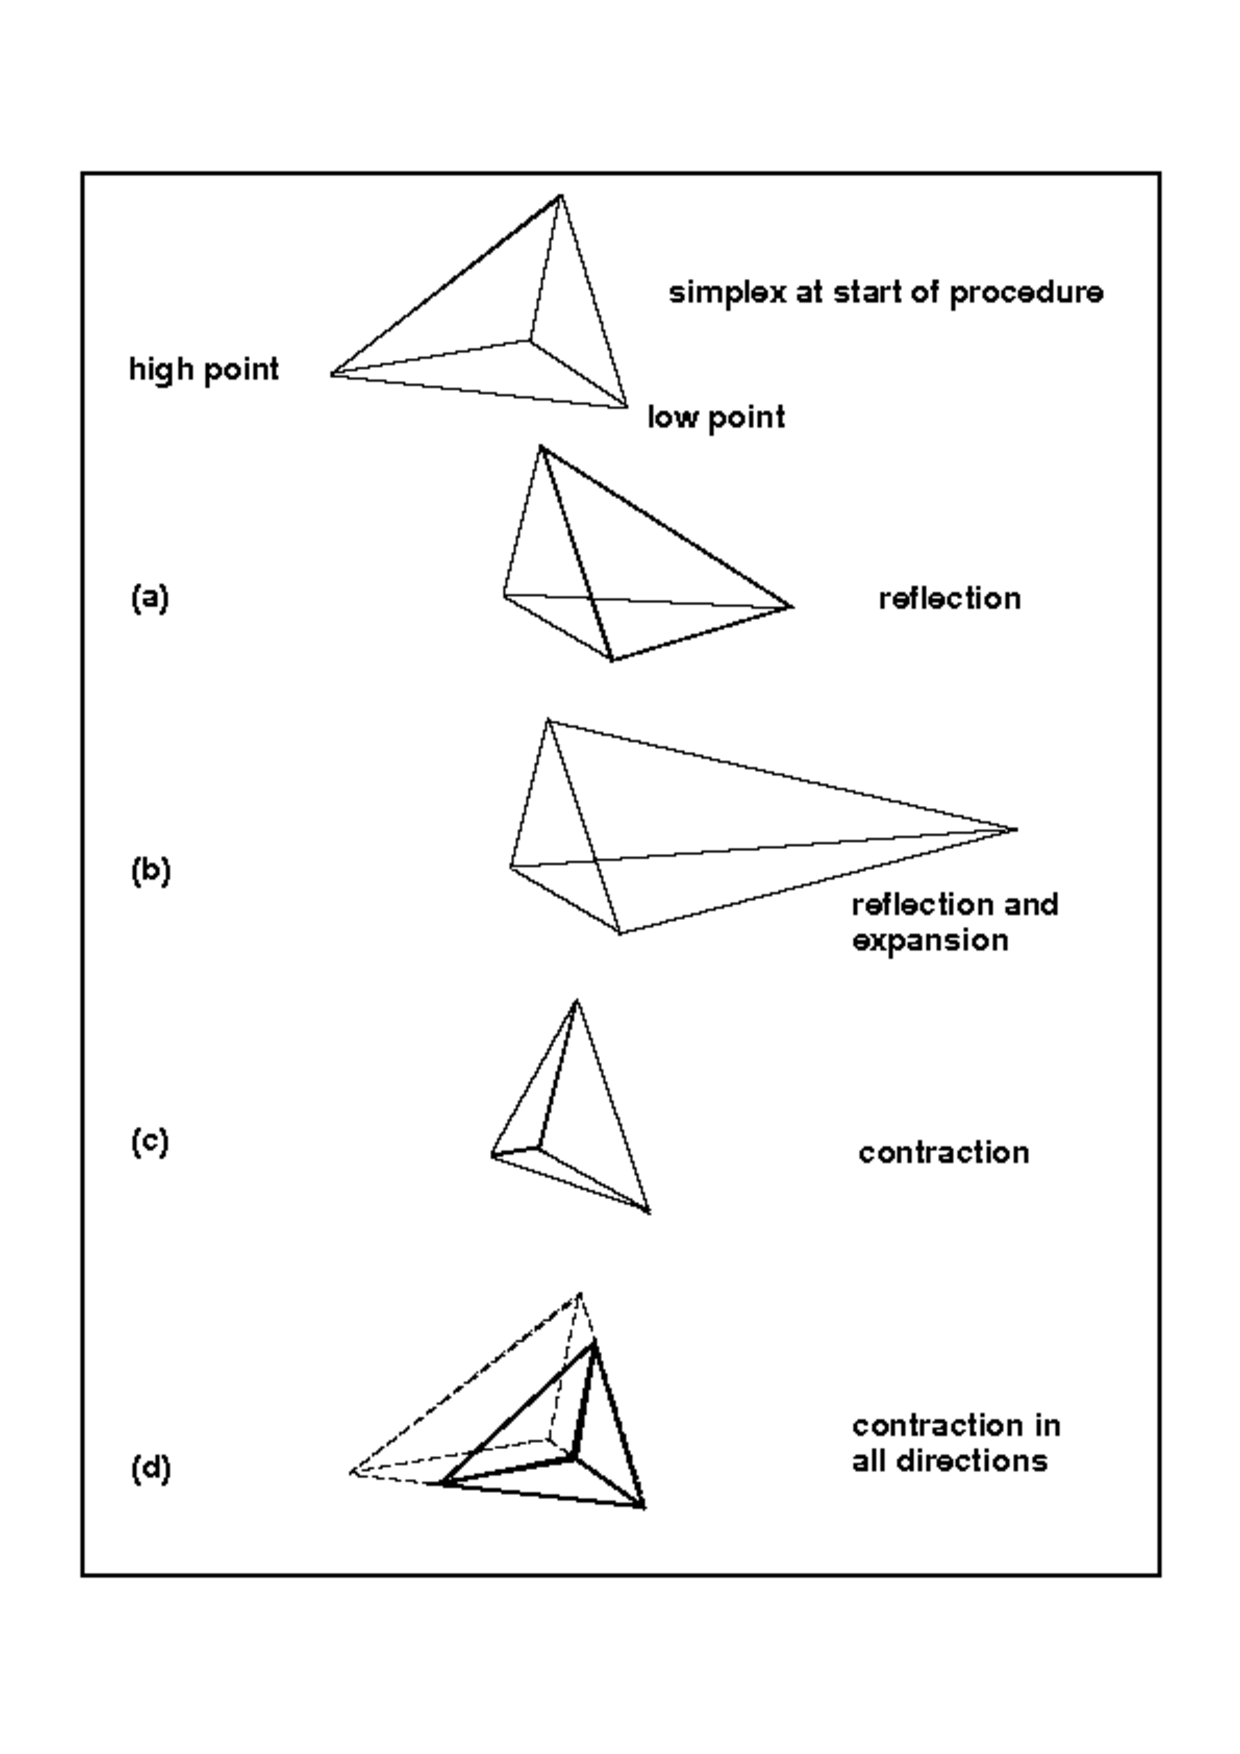
\includegraphics{image/neldermead.pdf}}

  \vspace*{-4em}
  \hspace*{16em}{\tiny\url{http://www.kniaz.net/software/RosNM.aspx}}
\end{frame}

\section{シミュレーテッド・アニーリング}

\begin{frame}[t,fragile]{確率過程を用いた最適化}
  \begin{itemize}
    \setlength{\itemsep}{1em}
  \item 最急降下法 (steepest decent)
    \begin{itemize}
    \item 初期状態をランダムに定める
    \item 配位を少しだけ変化させる
    \item エネルギー(コスト関数)が小さくなるなら採択、大きくなるなら棄却
    \item 状態が変化しなくなるまでくり返す $\Rightarrow$ 絶対零度でのMetropolis法
    \item 問題点 : エネルギー極小状態にすぐに捕まってしまう
    \end{itemize}
  \item 徐冷法 (simulated annealing)
    \begin{itemize}
    \item いきなり温度を零にするのではなく少しずつ下げていく
    \item どれくらいゆっくり下げれば良いか?
      \[
      T(t) \ge cN / \log(t+2)
      \]
    \item 実際には適当なスケジューリングで温度を下げ、何回か繰り返して最も良い結果を採択
    \end{itemize}
  \end{itemize}
\end{frame}

\begin{frame}[t,fragile]{最急降下法とシミュレーテッド・アニーリング}
  \noindent\resizebox{0.45\textwidth}{!}{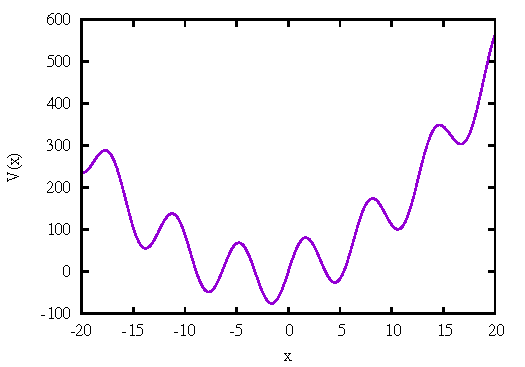
\includegraphics{image/potential.pdf}}

  \noindent\hspace*{.5em}\resizebox{0.43\textwidth}{!}{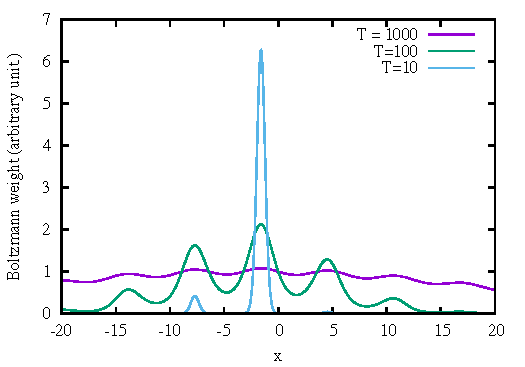
\includegraphics{image/boltzmann.pdf}}

  \vspace*{-17em}\hspace*{12.5em}\resizebox{0.6\textwidth}{!}{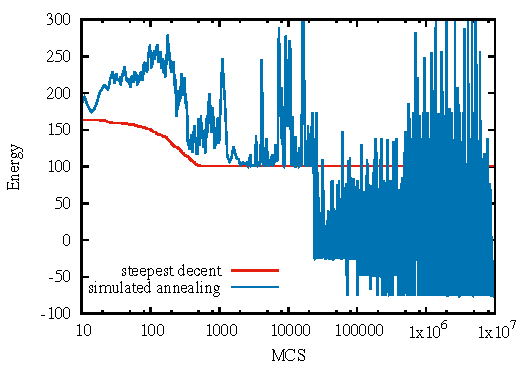
\includegraphics{image/energy.pdf}}

  \hspace*{17em}$T(t) = 100 - \frac{99}{10^7} t$
\end{frame}

\begin{frame}[t,fragile]{離散最適化問題への応用}
  \begin{itemize}
    \setlength{\itemsep}{1em}
  \item 微分を必要としないので、離散最適化問題にも適用可
    \begin{itemize}
    \item 例: 巡回セールスマン問題、数独、ナップザック問題
    \end{itemize}
  \item いかに状態とエネルギーを定義するかが重要
    \begin{itemize}
    \item 例: $n \times n$魔法陣 (行・列・ななめの和$M = n(n^2+1)/2$)
    \item 「状態」C: $1\sim n^2$の自然数をある順序でます目に並べたもの
    \item 「エネルギー」
      \[
      E(C) = \sum_{\rm row} (S_r-M)^2 + \sum_{\rm col} (S_c-M)^2 + \sum_{\rm diag} (S_d-M)^2
      \]
    \item 「正しい」魔方陣: $E(C) = 0$
    \end{itemize}
  \item 解の数(絶対零度のエントロピー)を求めるのにも利用できる
  \end{itemize}
\end{frame}


\section{}

\begin{frame}[t,fragile]{実習・講義予定}
  \begin{itemize}
    \setlength{\itemsep}{1em}
  \item 実習 EX6
    \begin{itemize}
    \item モンテカルロ法
    \item 最適化
    \end{itemize}
  \item 7/13 グループワーク発表会
    \begin{itemize}
    \item 発表会に関する連絡事項等はITC-LMSに掲載するので、適宜確認すること
    \end{itemize}
  \end{itemize}
\end{frame}

\end{document}
